%!TEX TS-program = lualatex
%!TEX encoding = UTF-8 Unicode

\documentclass[12pt, addpoints]{exam}
\usepackage[left=1in,right=0.75in,top=1in]{geometry}     

\printanswers

\usepackage{fontspec}
\def\mainfont{Linux Libertine O}
\setmainfont[Ligatures=TeX, Contextuals={NoAlternate}, BoldFont={* Bold}, ItalicFont={* Italic}, Numbers={OldStyle,Proportional}]{\mainfont}
%\setmonofont[Scale=MatchLowercase]{Inconsolata} 
\setsansfont[Scale=MatchLowercase]{Linux Biolinum O} 
\usepackage{microtype}

\usepackage{graphicx}
\graphicspath{%
	{/Users/goby/Pictures/teach/300/exams/}}%

% Used to get the last two digits of the year for the header below.
\def\short#1{\csname @gobbletwo\expandafter\endcsname\number#1}

\pagestyle{headandfoot}
\firstpageheader{Evolution, Exam 2, \textsc{s}\short{\year}.}{}{%
	\ifprintanswers\textbf{KEY}\else Name: \enspace \makebox[2.5in]{\hrulefill}\fi}
\runningheader{}{}{\small{pg. \thepage}}

\footer{\iflastpage{\small \rule{0.6in}{0.4pt} / \numpoints\ points}{}}{}{}%{\makebox[0.75in]{\hrulefill}}
\extrafootheight{-0.5in}

%\footer{}{}{}
%\extrafootheight{-0.5in}

\pointsinmargin
\marginpointname{ pts}
\marginbonuspointname{ pts \textsc{e.c.}}

\bonuspointpoints{point extra credit}{points extra credit}

\usepackage{multicol}
\usepackage{booktabs}
\usepackage{array}
\newcolumntype{L}[1]{>{\raggedright\let\newline\\\arraybackslash\hspace{0pt}}p{#1}}
\newcolumntype{C}[1]{>{\centering\let\newline\\\arraybackslash\hspace{0pt}}p{#1}}
\newcolumntype{R}[1]{>{\raggedleft\let\newline\\\arraybackslash\hspace{0pt}}p{#1}}

%% Remove comment %% to print answer key.
\unframedsolutions
\renewcommand{\solutiontitle}{}
\SolutionEmphasis{\bfseries}


\newcommand*\AnswerBox[2]{%
	\parbox[t][#1]{0.92\textwidth}{%
		\begin{solution}#2\end{solution}}
	\vspace{\stretch{1}}
}

\newenvironment{AnswerPage}[1]
{\begin{minipage}[t][#1]{0.92\textwidth}%
		\begin{solution}}
		{\end{solution}\end{minipage}
	\vspace{\stretch{1}}}

\newlength{\basespace}
\setlength{\basespace}{5\baselineskip}


\begin{document}

\begin{questions}

\question[3]
Explain co-option of genes. Provide an example.

	\AnswerBox{0.15\textheight}{%
		Co-option is when a gene evolves a new function while retaining an existing function. Examples include \emph{Hox} genes and tetrapod appendages, toolkit genes for eye spots, non-toolkit genes for crystallin proteins.}

\question
The longnose butterflyfish (right, on screen) has an unusually long mouth compared to other species of butterflyfishes (left). You plan to study the genetics of jaw length in the butterflyfishes.  
\begin{parts}
	\part[2] Identify one toolkit gene that you would be wise to study first.
	
	\AnswerBox{0.01\textheight}{Ca\textsc{m}1}

	\part[5] Explain the existing evidence that caused you to identify this toolkit gene.
	
	\AnswerBox{0.15\textheight}{%		
		Ca\textsc{m}1 was shown to correlate with jaw length in birds, may also work in fishes.
	}

\end{parts}

\question[5]
Describe how thermoregulation might have favored the evolution of bipedalism in hominin ancestors.

\AnswerBox{0.15\textheight}{Reduce sun shining on back, increase exposure to breeze.}


\bonusquestion[2]
	Name two of the maternal effect genes that control the earliest development of the Drosophila egg, before \emph{Hox} genes are used.
	
	\ifprintanswers\textbf{Nanos, Bicoid, Hunchback, Caudal}\fi


\newpage


\question[5]
Are dinosaurs extinct?  Explain why or why not.  Apply the concept of monophyly to justify your explanation.

\AnswerBox{2\basespace}{No, birds are dinosaurs. Birds are more closely related to theropod dinosaurs than theropods are to other dinosaurs (they share a more recent common ancestor). If theropods are dinosaurs, then so must be birds.}

\question[5]
Whales are most closely related to hippopotamuses but lack rear limbs.  Explain how a change to \emph{Hox} gene expression might cause the loss of rear limbs. 

	\AnswerBox{2\basespace}{%
	Mutations to \emph{Hox} A and \emph{Hox} D 9-13 may have stopped limb production. Or, \emph{Hox} genes for the a-p axis may have stopped producing legs in the posterior end.
	}


\question[5]
Explain ecological release and how it might have contributed to the Cambrian radiation.

	\AnswerBox{2\basespace}{%
	The Ediacaran fauna occupied various ecological niches. The extinction of the Ediacaran fauna would have freed up ecological resources, allowing the Cambrian fauna to evolve into new niches.}



\newpage

\question[10]
The snapping shrimp \textit{Synalpheus brooksi} lives in sponges on coral reefs.  Duffy (1996) showed that shrimp occupying nearby but different species of sponges rarely come into contact with each other because they don't usually leave their sponges. In the lab, a male shrimp from one sponge species is extremely aggressive towards females from a different sponge species, suggesting reproductive incompatibility. Analyses showed that shrimp from the same sponge species were genetically similar but shrimp from different sponge species were genetically distinct. Duffy argued the shrimp in different sponges are different species.  If so, explain which prezygotic mechanism or mechanisms reproductively isolate shrimps in different sponge species.

\AnswerBox{0.3\textheight}{%
	Ecological. Occupy different habitats.
}

\question[10]
The grasses (Poaceae, includes rice and corn) produce flowers that lack petals and sepals but have stamens and carpels.  Given the three classes of \textsc{mads} genes below, which class or classes most likely had a mutation or change in expression that caused the loss of petals and sepals?  Draw the ABC model of floral development, and then use that model to justify your answer.  Class A: Apetala1.  Class B: Apetala3.  Class C: Agamous.

	\begin{AnswerPage}{0.3\textheight}
	Class A causes loss of sepals and petals. Class B and C form stamens and C alone forms carpals. A needed for both petals and sepals. 
	\end{AnswerPage}

\newpage


\question[15]

\begin{multicols}{2}
\flushleft
The table at right (Sharp et al. 2005) shows how \textit{E. coli} uses 32 codons from 40 highly expressed genes. The tabled numbers are the ratio of actual use to expected use if all codons were used equally. A ratio of 1 means the codon is used exactly as often as expected (e.g., Met, in bold). Explain whether the data in the table provide evidence for natural selection at the genetic level. Explain why or why not. Use 1--2 specific codons from the table to support your answer.
\columnbreak
\begin{tabular}{@{}llrcllr@{}}
	\toprule
	\multicolumn{7}{l}{Codon use in \textit{E. coli}.}\\
	\midrule
	Phe & UUU & 0.45 &  & Ser & UCU & 2.54\\
Phe & UUC & 1.55 &  & Ser & UCC & 1.52\\
Leu & UUA & 0.14 &  & Ser & UCA & 0.19\\
Leu & UUG & 0.25 &  & Ser & UCG & 0.06\\
Leu & CUU & 0.30 &  & Pro & CCU & 0.59\\
Leu & CUC & 0.23 &  & Pro & CCC & 0.05\\
Leu & CUA & 0.01 &  & Pro & CCA & 0.52\\
Leu & CUG & 5.07 &  & Pro & CCG & 2.85\\
Ile & AUU & 0.72 &  & Thr & ACU & 1.89\\
Ile & AUC & 2.27 &  & Thr & ACC & 1.75\\
Ile & AUA & 0.01 &  & Thr & ACA & 0.19\\
\textbf{Met} & \textbf{AUG} & \textbf{1.00} &  & Thr & ACG & 0.17\\
Val & GUU & 2.07 &  & Ala & GCU & 1.83\\
Val & GUC & 0.30 &  & Ala & GCC & 0.32\\
Val & GUA & 1.14 &  & Ala & GCA & 1.09\\
Val & GUG & 0.48 &  & Ala & GCG & 0.76\\
	\bottomrule
	\end{tabular}
\end{multicols}
%	\end{minipage}
	\begin{solution}
	Codon bias is present.
	\end{solution}

\newpage

\question[10]
{\addfontfeatures{Numbers=Lining}
Use the following matrix of homologies (C1\dots C8) to make a phylogenetic tree that shows the relationships of the nine taxa (T1\dots T9). Only one tree is possible. Mark each branch with the homology that unites those taxa into a clade. You do not have to draw the outgroup. %The outgroup is not shown but is presumed to have character state 0 for all characters.

\begin{tabular}{@{}rcccccccc@{}}
\toprule
 & C1 & C2 & C3 & C4 & C5 & C6 & C7 & C8 \\
\midrule
T1 & 0 & 1 & 1 & 0 & 1 & 0 & 0 & 0 \\
T2 & 0 & 1 & 1 & 1 & 0 & 1 & 0 & 1 \\
T3 & 0 & 1 & 1 & 1 & 0 & 1 & 1 & 1 \\
T4 & 0 & 1 & 1 & 1 & 0 & 0 & 0 & 1 \\
T5 & 0 & 1 & 1 & 0 & 1 & 0 & 0 & 0 \\
T6 & 1 & 0 & 1 & 0 & 0 & 0 & 0 & 0 \\
T7 & 0 & 1 & 1 & 1 & 0 & 0 & 0 & 0 \\
T8 & 0 & 1 & 1 & 1 & 0 & 1 & 1 & 1 \\
T9 & 1 & 0 & 1 & 0 & 0 & 0 & 0 & 0 \\
\bottomrule
\end{tabular}
}

\ifprintanswers
 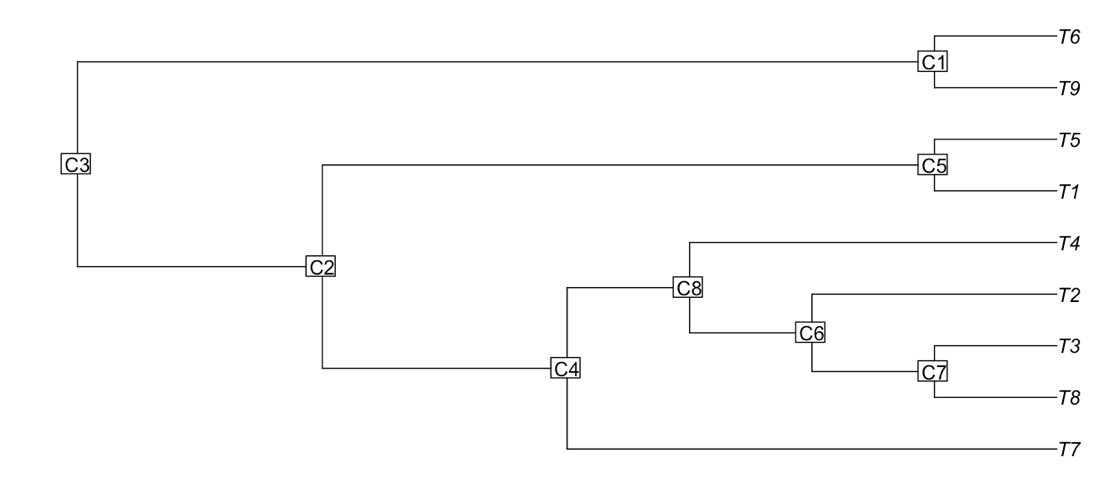
\includegraphics[width=0.75\textwidth]{phylogeny_answer.png}
\fi

\end{questions}

\end{document}